\documentclass[titlepage, letterpaper, fleqn]{article}
\usepackage[utf8]{inputenc}
\usepackage{fancyhdr} % fancy headers, of course!
\usepackage{amsmath} % what do you think?
\usepackage{amsthm} % theorems!
\usepackage{extramarks} % more cute things
\usepackage{enumitem} % i'm not sure...
\usepackage{multicol} % multicolumn...?
\usepackage{amssymb} % more symbols
\usepackage{booktabs} % cool looking tables
\usepackage{tikz} %venn and shizzle
\usepackage{tikz-qtree-compat} %tableaux
\usepackage{lipsum} %lorem ipsum dolor sit amet f u
\usepackage{mathrsfs} %math script for calligraphic scripting, I GUESS

\topmargin=-0.45in
\evensidemargin=0in
\oddsidemargin=0in
\textwidth=6.5in
\textheight=9.0in
\headsep=0.25in


%
% You should change this things~
%

\newcommand{\mahteacher}{Dr. Viacheslav Kalashnikov}
\newcommand{\mahclass}{Applied Mathematics}
\newcommand{\mahtitle}{Topic II - Activity 9}
\newcommand{\mahdate}{September 28, 2016}
\newcommand{\spacepls}{\vspace{5mm}}
\renewcommand\qedsymbol{\(\blacksquare\)}

%
% Header markings
%

\pagestyle{fancy}
\lhead{1170065 - Xavier Sánchez}
\chead{}
\rhead{}
\lfoot{}
\rfoot{}


\renewcommand\headrulewidth{0.4pt}
\renewcommand\footrulewidth{0.4pt}

\setlength\parindent{0pt}


%
% Create Problem Sections (stolen directly from jdavis/latex-homework-template @ github!)
%

\newcommand{\enterProblemHeader}[1]{
\nobreak\extramarks{}{Problem \arabic{#1} continued on next page\ldots}\nobreak{}
\nobreak\extramarks{Problem \arabic{#1} (continued)}{Problem \arabic{#1} continued on next page\ldots}\nobreak{}
}

\newcommand{\exitProblemHeader}[1]{
\nobreak\extramarks{Problem \arabic{#1} (continued)}{Problem \arabic{#1} continued on next page\ldots}\nobreak{}
\stepcounter{#1}
\nobreak\extramarks{Problem \arabic{#1}}{}\nobreak{}
}

\setcounter{secnumdepth}{0}
\newcounter{partCounter}
\newcounter{homeworkProblemCounter}
\setcounter{homeworkProblemCounter}{1}
\nobreak\extramarks{Exercise \arabic{homeworkProblemCounter}}{}\nobreak{}

% Alias for the Solution section header
\newcommand{\solution}{\textbf{\Large Solution}}

%Alias for the new step section
\newcommand{\steppy}[1]{\textbf{\large #1}}

%
% Homework Problem Environment
%
% This environment takes an optional argument. When given, it will adjust the
% problem counter. This is useful for when the problems given for your
% assignment aren't sequential. See the last 3 problems of this template for an
% example.
%
\newenvironment{homeworkProblem}[1][-1]{
\ifnum#1>0
\setcounter{homeworkProblemCounter}{#1}
\fi
\section{Exercise \arabic{homeworkProblemCounter}}
\setcounter{partCounter}{1}
\enterProblemHeader{homeworkProblemCounter}
}{
\exitProblemHeader{homeworkProblemCounter}
}

%
% Venn diagrams defs
%

% \def\firstcircle{(0,0) circle (1.5cm)}
% \def\secondcircle{(0:2cm) circle (1.5cm)}
% \colorlet{circle edge}{blue!50}
% \colorlet{circle area}{blue!20}

% \tikzset{filled/.style={fill=circle area, draw=circle edge, thick},
%     outline/.style={draw=circle edge, thick}}

%
% My actual info
%

\title{
\vspace{1in}
\textbf{Tecnológico de Monterrey} \\
\vspace{0.5in}
\textmd{\mahclass} \\
\large{\textit{\mahteacher}} \\
\vspace{0.5in}
\textsc{\mahtitle}\\
\textsc{2.3.1 Natural Deduction}\\
\textsc{2.3.2 Propositional Logic}\\
\textsc{2.3.3 Propositional Logic}\\
\author{01170065  - MIT \\
Xavier Fernando Cuauhtémoc Sánchez Díaz \\
\texttt{mail@gmail.com}}
\date{\mahdate}
}

\begin{document}

\begin{titlepage}
\maketitle
\end{titlepage}

%
% Actual document starts here~
%

\section{Exercise 2.3.1}

{\large \textbf{a)} Show that \(\forall x p(x) \wedge \forall x q(x) \implies \forall x (p(x) \wedge q(x))\) is a valid formula.}

\spacepls

This formula is valid since universal quantifiers are distributable over conjunction in both ways. Nevertheless, proof is as follows.

\begin{proof}
The converse of this implication is unsatisfiable.

\begin{align*}
& \neg (\forall x p(x) \wedge \forall x q(x) \implies \forall x (p(x) \wedge q(x))) = & \tag*{Converse}
\\ & = \neg (\neg (\forall x p(x) \wedge \forall x q(x)) \vee \forall x (p(x) \wedge q(x))) &\tag*{Material implication}
\\ & = (\forall x p(x) \wedge \forall x q(x)) \wedge \neg \forall x (p(x) \wedge q(x)) &\tag*{de Morgan}
\\ & = \forall x p(x) \wedge \forall x q(x) \wedge \exists x \neg (p(x) \wedge q(x)) &\tag*{Negation of \(\forall\) is \(\exists \neg\)}
\\ & = \forall x p(x) \wedge \forall x q(x) \wedge \exists x (\neg p(x) \vee \neg q(x)) &\tag*{de Morgan}
\\ & = \forall x p(x) \wedge \forall x q(x) \wedge (\exists x \neg p(x) \vee \exists x \neg q(x)) &\tag*{\(\exists\) is distributive over \(\vee\)}
\\ & = (\forall x p(x) \wedge \forall x q(x) \wedge \exists x \neg p(x)) \vee (\forall x p(x) \wedge \forall x q(x) \wedge \exists x \neg q(x)) &\tag*{\(\wedge\) is distributive over \(\vee\)}
\end{align*}

And since both \(\forall x p(x) \wedge \forall x q(x) \wedge \exists x \neg p(x)\) and \(\forall x p(x) \wedge \forall x q(x) \wedge \exists x \neg q(x))\) are contradictions, then the converse is unsatisfiable, and thus the original formula is valid.
\end{proof}

\spacepls

{\large \textbf{b)} Show that \(\forall x (p(x) \implies q(x)) \implies (\forall x p(x) \implies \forall x q(x))\) is a valid formula but its converse \((\forall x p(x) \implies \forall x q(x)) \implies \forall x (p(x) \implies q(x))\) is not.}

\spacepls

To show the validity of the first part of the exercise, proving the converse suffices.
\begin{proof}
\begin{align*}
&\neg(\forall x (p(x) \implies q(x)) \implies (\forall x p(x) \implies \forall x q(x))) & \tag*{Converse}
\\ & = \neg(\neg (\forall x (p(x) \implies q(x))) \vee (\forall x p(x) \implies \forall x q(x))) & \tag*{Material implication}
\\ & = \forall x (p(x) \implies q(x)) \wedge \neg (\forall x p(x) \implies \forall x q(x)) & \tag*{de Morgan}
\\ & =\forall x (\neg p(x) \vee q(x)) \wedge \neg(\neg \forall x p(x) \vee \forall x q(x)) & \tag*{Material implication}
\\ & =\forall x (\neg p(x) \vee q(x)) \wedge \forall x p(x) \vee \neg \forall x q(x) & \tag*{de Morgan}
\\ & = \neg \exists x \neg (\neg p(x) \vee q(x)) \wedge \forall x p(x) \vee \neg \forall x q(x) & \tag*{Duality of quantifiers}
\\ & = \neg \exists x (p(x) \wedge \neg q(x)) \wedge \forall x p(x) \vee \neg \forall x q(x) & \tag*{de Morgan}
\\ & = \neg \exists x p(x) \wedge \neg \exists x \neg q(x) \wedge \forall x p(x) \vee \neg \forall x q(x) & \tag*{\(\exists\) distributes over \(\wedge\)}
\\ & = \neg \exists x p(x) \wedge \neg \exists x \neg q(x) \wedge \forall x p(x) \wedge \exists x \neg q(x) & \tag*{Duality of quantifiers}
\\ & = \neg \exists x p(x) \wedge \forall x p(x) \wedge \neg \exists x \neg q(x) \wedge \exists x \neg q(x) & \tag*{\(\wedge\) is commutative}
\end{align*}
And since both \(\neg \exists x p(x) \wedge \forall x p(x)\) and \(\neg \exists x \neg q(x) \wedge \exists x \neg q(x)\) are contradictions, then the converse is unsatisfiable, and thus the original formula is valid.
\end{proof}

\spacepls

The second part of the exercise can be falsified using a counterexample:

\begin{proof}
Let \(x\) be any piece in a chess game where I'm playing the white pieces, \(p(x)\) mean ``\(x\) is a white'' and \(q(x)\) mean ``\(x\) is a piece I own''.

Then, \(\forall x(p(x) \implies q(x))\) means ``all white pieces are my pieces'' which is true.

However, \(\forall x p(x) \implies \forall x q(x)\) means ``if all pieces are white, then all pieces are mine'', which is not true since there could be pieces that are not mine (i.e. black pieces) even if all white pieces are in my possession.

So the implication \((\forall x p(x) \implies \forall x q(x)) \implies \forall x (p(x) \implies q(x))\) is falsifiable.
\end{proof}

\section{Exercise 2.3.2}

{\large \textbf{a)} Prove that \((\forall x p(x) \implies \forall x q(x)) \implies \forall x (p(x) \implies q(x))\) is not valid by constructing a semantic tableau for its negation.}

\spacepls
\begin{proof}
The following tableau corresponds to the negation of \((\forall x p(x) \implies \forall x q(x)) \implies \forall x (p(x) \implies q(x))\).
\spacepls

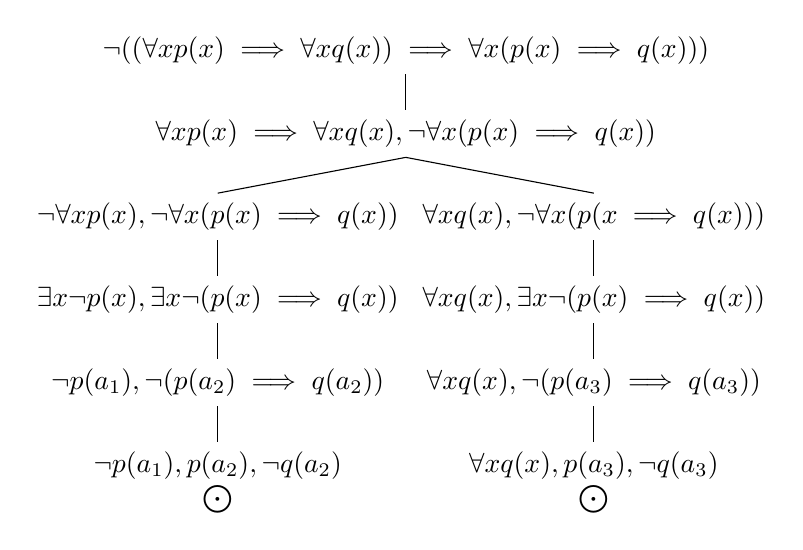
\begin{tikzpicture}
\tikzset{every tree node/.style={align=center,anchor=north}}
\tikzset{grow'=down}
\Tree [.{$\neg ((\forall x p(x) \implies \forall x q(x)) \implies \forall x (p(x) \implies q(x)))$}  
    [.{$\forall x p(x) \implies \forall x q(x), \neg \forall x (p(x) \implies q(x))$} [
    .{$\forall x q(x), \neg \forall x (p(x \implies q(x)))$} [.{$\forall x q(x), \exists x \neg (p(x) \implies q(x))$} [.{$\forall x q(x), \neg (p(a_3) \implies q(a_3))$} 
    {$\forall x q(x), p(a_3), \neg q(a_3)$}\\{$\bigodot$} ] ] ]
    [.{$\neg \forall x p(x), \neg \forall x (p(x) \implies q(x))$} 
    [.{{$\exists x \neg p(x), \exists x \neg (p(x) \implies q(x))$}} 
    [.{$\neg p(a_1), \neg (p(a_2) \implies q(a_2))$} {$\neg p(a_1), p(a_2), \neg q(a_2)$}\\{$\bigodot$} ] ] ] ] ]
\end{tikzpicture}

\spacepls

The right branch is considered finite and open since there's a universally quantified formula. And since there are open branches, then the original formula is falsifiable.
\end{proof}

\section{Exercise 2.3.3}

{\large \textbf{a)} Prove that \(\exists x (A(x) \implies B(x)) \iff (\forall x A(x) \implies \exists x B(x))\) is valid.}

\spacepls

\(\exists x (A(x) \implies B(x))\) is logically equivalent to \((\forall x A(x) \implies \exists x B(x))\), so this formula is valid.

\begin{proof}
\begin{align*}
& \exists x (A(x) \implies B(x)) = &
\\ & = \exists x (\neg A(x) \vee B(x)) & \tag*{Material implication}
\\ & = \exists x \neg A(x) \vee \exists x B(x) & \tag*{$\exists$ distributes over $\vee$}
\\ & = \neg \forall x A(x) \vee \exists x B(x) & \tag*{Duality of quantifiers}
\\ & = \forall x A(x) \implies \exists x B(x) & \tag*{Material implication}
\end{align*}
\begin{align*}
& \forall x A(x) \implies \exists x B(x) = &
\\ & = \neg \forall x A(x) \vee \exists x B(x) & \tag*{Material implication}
\\ & = \exists x \neg A(x) \vee \exists x B(x) & \tag*{Duality of quantifiers}
\\ & = \exists x (\neg A(x) \vee B(x)) & \tag*{$\exists$ distributes over $\vee$}
\\ & = \exists x (A(x) \implies B(x)) & \tag*{Material implication}
\end{align*}
\end{proof}

\pagebreak

{\large \textbf{b)} Prove that \((\exists x A(x) \implies \forall x B(x)) \implies \forall x (A(x) \implies B(x))\) is valid.}

\spacepls

\begin{proof}
\begin{align*}
& (\exists x A(x) \implies \forall x B(x)) = &
\\ & = \neg \exists A(x) \vee \forall x B(x) & \tag*{Material implication}
\\ & = \forall x \neg A(x) \vee \forall x B(x) & \tag*{Duality of quantifiers}
\\ & = \forall x (\neg A(x) \vee B(x)) & \tag*{$\forall$ distributes over $\vee$}
\\ & = \forall x (A(x) \implies B(x)) & \tag*{Material implication}
\end{align*}
\(\exists x A(x) \implies \forall x B(x)\) can be expressed as \(\forall x (A(x) \implies B(x))\), therefore the formula is valid.
\end{proof}

\spacepls

{\large \textbf{c)} Prove that \(\forall x (A(x) \vee B(x)) \implies (\forall x A(x) \vee \exists x B(x))\) is valid.}

\spacepls

\begin{proof}
The converse of this implication is unsatisfiable.
\begin{align*}
& \neg (\forall x (A(x) \vee B(x)) \implies (\forall x A(x) \vee \exists x B(x))) = & \tag*{Converse}
\\ & = \forall x (A (x) \vee B(x)) \wedge \neg (\forall x A(x) \vee \exists x B(x)) & \tag*{Material implication \& de Morgan}
\\ & = \forall x (A (x) \vee B(x)) \wedge \neg \forall x A(x) \wedge \neg \exists B(x) & \tag*{de Morgan}
\\ & = \neg \exists x \neg (A(x) \vee B(x)) \wedge \neg \forall x A(x) \wedge \neg \exists B(x) & \tag*{Duality of quantifiers}
\\ & = \neg \exists x (\neg A(x) \wedge \neg B(x)) \wedge \neg \forall x A(x) \wedge \neg \exists B(x) & \tag*{de Morgan}
\\ & = \neg \exists x \neg A(x) \wedge \neg \exists x \neg B(x) \wedge \forall x A(x) \wedge \neg \exists x B(x) & \tag*{$\exists$ distributes over $\wedge$}
\\ & = \neg \exists x \neg A(x) \wedge \forall x B(x) \wedge \forall x A(x) \wedge \neg \exists x B(x) & \tag*{Duality of quantifiers}
\end{align*}
Since \(\forall x B(x) \wedge \neg \exists x B(x)\) is a contradiction, this converse is unsatisfiable.

Therefore, the original formula is valid.
\end{proof}

\spacepls

{\large \textbf{d)} Prove that \(\forall x (A(x) \implies B(x)) \implies (\exists x A(x) \implies \exists x B(x))\) is valid.}

\spacepls

\begin{proof}
The converse of this implication is unsatisfiable.
\begin{align*}
& \neg (\forall x (A(x) \implies B(x)) \implies (\exists x A(x) \implies \exists x B(x))) = & \tag*{Converse}
\\ & = \forall x (A (x) \implies B(x)) \wedge \neg (\exists x A(x) \implies \exists x B(x)) & \tag*{Material implication \& de Morgan}
\\ & = \forall x (A(x) \implies B(x)) \wedge \exists x A(x) \wedge \neg \exists x B(x) & \tag*{Material implication \& de Morgan}
\\ & = \neg \exists \neg (A(x) \implies B(x)) \wedge \exists x A(x) \wedge \neg \exists x B(x) & \tag*{Duality of quantifiers}
\\ & = \neg \exists x (A(x) \wedge \neg B(x)) \wedge \exists x A(x) \wedge \neg \exists x B(x) & \tag*{Material implication \& de Morgan}
\\ & = \neg \exists x A(x) \wedge \neg \exists x \neg B(x) \wedge \exists x A(x) \wedge \neg \exists x B(x) & \tag*{$\exists$ distributes over $\wedge$}
\\ & = \neg \exists x A(x) \wedge \forall x B(x) \wedge \exists x A(x) \wedge \neg \exists x B(x) & \tag*{Duality of quantifiers}
\end{align*}
Since \(\neg \exists x A(x) \wedge \exists x A(x)\) and \(\forall x B(x) \wedge \neg \exists x B(x)\) are contradictions, this converse is unsatisfiable.

Therefore, the original formula is valid.
\end{proof}
\end{document}